\subsection{Five-direction groups with matched Vanilla controls}\label{app:width5}
Run \texttt{95fbab1d48bf} compares five-direction GGF and Vanilla across
the declared training starts with the saved four-direction cap-0.40 models. It reuses the
same 2,000 training, 400 development, and 1,500 inspected test
images, frozen backbone, normalization, category set, and scoring rules.
All six new endpoints freeze before test scoring. The main configuration is
GGF, trained with ordinary gradients.

\paragraph{Initialization and capacity.}
For each of 75 categories, preserve the four saved starting directions
byte-for-byte. Recompute its training foreground outer-product matrix,
verify agreement with the leading four-dimensional eigenspace, and append
the fifth eigen-direction after projecting away the saved four. Normalize
its length and orient its sign using training projection energy. Foreground
coverage is at least 50\%. Crowd coverage is at most 10\%. Neither development
nor test features determine these axes. The remaining 949 groups are random.
The category initializer is shared across seeds, while reserve directions
and training order vary.

Both 5D arms have 1,024 groups, 5,120 directions, Top-16 gating, and at most
80 active coefficients. They contain 7,869,440 encoder/decoder parameters,
25\% more than width four's 6,295,552, including encoder biases. Guided
learning adds 150 logistic-classifier-head parameters. Equal updates therefore do not
imply equal parameter capacity, activity budget, or computation across widths.
Within width five, Vanilla controls group size and activity but differs in
mask initialization and supervision.

\paragraph{Matched training and fixed readouts.}
Each arm receives a new 40-epoch, 7,640-update reconstruction warm-up.
Continuation starts from its minimum-development-MSE warm-up checkpoint,
not necessarily update 7,640. TRAIN-only contrast and detection readouts
are then fixed. Different warm-ups can select different groups. Mask GGF
and Vanilla each receive 2,500 plus 500 updates, totaling 10,640 scheduled
updates. Model Adam resets at the phase boundary. Guided heads and the
adaptive controller carry forward. Guided learning retains the same bounded
controller, contrast range $[0.0125,0.40]$, detection range $[0.0025,0.40]$,
and reconstruction weight one. The upper bound is a cap, not a fixed weight.
Vanilla trains reconstruction only. Both retain learning rate
$3\times10^{-4}$, eight images per update, noise scale 0.1, and gradient
clipping at five during continuation.

Warm-up patch permutations and noise schedules match across widths and
arms. The guided-phase streams use seeds $71{,}000+s$ and $82{,}000+s$,
where $s$ is the training seed. Saved hash chains verify these schedules.
The frozen four-direction controls and their test audits are reused rather
than retrained. The new work is six warm-ups and six 3,000-update fits,
or 63,840 model updates. Final endpoints are scored regardless of eligibility.

\begin{table*}[t]\centering\small
\caption{Values with $\pm$ show mean and sample SD. Width-four/five test means (\%). All rows pass the original
native-reference development-MSE allowance in all runs.}
\label{tab:width5-means}
\begin{tabular}{@{}lrrr@{}}\hline
Model & Capture & Patch AP & VE\\\hline
GGF 4: cap 0.40 & $38.83\pm0.04$ & $75.19\pm0.25$ & $65.38\pm0.05$\\
GGF 5: cap 0.40 & $39.43\pm0.15$ & $75.04\pm0.42$ & $66.67\pm0.05$\\
Vanilla BSF 4 & $21.31\pm0.49$ & $57.35\pm0.83$ & $66.74\pm0.05$\\
Vanilla BSF 5 & $22.30\pm0.53$ & $59.59\pm1.66$ & $68.12\pm0.10$\\\hline
\end{tabular}\end{table*}

\begin{agfresulttable}
\caption{All five-direction endpoints: test percentages.}
\label{tab:width5-seeds}
\begin{tabular}{@{}rlrrr@{}}\hline
Seed & Model & Capture & AP & VE\\\hline
21 & GGF 5 &39.470&75.501&66.617\\
21 & Vanilla 5 &22.488&58.815&68.051\\
22 & GGF 5 &39.559&74.686&66.690\\
22 & Vanilla 5 &21.701&58.452&68.226\\
23 & GGF 5 &39.270&74.942&66.709\\
23 & Vanilla 5 &22.706&61.487&68.070\\\hline
\end{tabular}\end{agfresulttable}

\paragraph{Outcomes and uncertainty.}
Widening GGF improves mean Capture by 0.60 points and VE by 1.29 points.
Both gains occur in every run, and each Capture interval lies above zero.
Mean AP falls by 0.15 points: seed 21 improves, seeds 22 and 23 decline.
Only seed 23's AP-change interval excludes zero, in the negative direction.
Against matched 5D Vanilla, GGF gains 17.13 Capture and 15.46 AP points,
with positive intervals in every run, but loses 1.44 VE points. Widening
Vanilla improves all three means too: 0.98 Capture, 2.24 AP, and 1.38 VE points.
Its Capture intervals are positive in all seeds. Its AP interval is positive
only in seed 23.

Nine paired comparisons use 200 whole-image bootstrap draws. Intervals
condition on fitted models and omit seed-level, selection, and multiplicity
uncertainty. VE changes are point estimates. Native eligibility uses the
unchanged development-MSE limit, separately from test VE. Test scores remain
distinct from development means of 39.14\% Capture, 80.60\% AP, and 66.20\% VE.

\begin{agfresulttable}
\caption{All 5D-study paired 95\% image intervals (percentage points).
G5/G4 denote guided models. V5/V4 denote Vanilla.}
\label{tab:width5-intervals}
\begin{tabular}{@{}rlrr@{}}\hline
Seed & Comparison & Capture interval & AP interval\\\hline
21 & G5--V5 & [16.57,17.44] & [15.20,17.89]\\
22 & G5--V5 & [17.37,18.36] & [14.81,17.52]\\
23 & G5--V5 & [16.12,16.95] & [12.20,14.38]\\
21 & G5--G4 & [0.53,0.75] & [$-0.09$,0.71]\\
22 & G5--G4 & [0.59,0.79] & [$-0.66$,0.12]\\
23 & G5--G4 & [0.39,0.59] & [$-1.06$,$-0.01$]\\
21 & V5--V4 & [0.36,0.99] & [$-0.44$,2.71]\\
22 & V5--V4 & [0.49,1.25] & [$-0.76$,2.42]\\
23 & V5--V4 & [1.19,1.77] & [3.80,6.54]\\\hline
\end{tabular}\end{agfresulttable}

Complete per-category reports, all intervals, endpoint identities,
initialization checks and development histories are in
\path{evidence/width5/}. Evaluation initially stopped after seed 21 because
the destination lacked copied 4D control audits. Recovery verified and
restored those immutable audits from the completed continuation source.
It changed no trained weights, readouts, test images, or numerical rules.
The completed width-five stage is independent of the two proposed, unrun stages
in the original notebook. The archive's global completion flag does not
indicate completion of those other experiments.

\subsection{Four-direction continuation}\label{app:continuation}
Run \texttt{32dcb7bd6e9c} adds 3,000 updates to cap-0.40 width-four
GGF and Vanilla, totaling 13,640 scheduled updates. The guided arms use
ordinary gradients or weighted encoder-only PCGrad~\citep{yu2020pcgrad}.
All preserve saved model and optimizer state, trained heads, controller,
fixed readouts, Top-16 gating, and matched new image/noise schedules.
Learning rate remains $3\times10^{-4}$ and noise scale 0.1. No warm-up or feature
extraction is repeated. Decoder gradients remain ordinary
weighted sums in this projection ablation.

All nine endpoints freeze before scoring the same cached 1,500 images.
Ordinary continuation gains 1.44 Capture points, but loses 0.17 AP and
0.55 VE points. Both guided continuations fail the original
development-MSE allowance in every run. Projection adds 0.12 Capture points
over ordinary continuation while reducing AP and VE, so it is not adopted.
Table~\ref{tab:continuation-means} retains its outcome. Complete per-seed
reports, all 18 paired comparisons, development histories, and frozen
identities remain in \path{evidence/continuation/}. Intervals use 200 whole-image draws under Appendix~\ref{app:secondary}.

\begin{table*}[t]\centering\small
\caption{Values with $\pm$ show mean and sample SD. Continuation test means (\%). Passes refer to the original
development-MSE allowance. Starting rows precede the 3,000 additional updates.}
\label{tab:continuation-means}
\begin{tabular}{@{}lrrrr@{}}\hline
Model & Capture & AP & VE & Passes\\\hline
GGF: start & $38.83\pm0.04$ & $75.19\pm0.25$ & $65.38\pm0.05$ & 3/3\\
GGF: continued & $40.28\pm0.15$ & $75.02\pm0.21$ & $64.83\pm0.01$ & 0/3\\
GGF: PCGrad & $40.40\pm0.14$ & $74.92\pm0.19$ & $64.73\pm0.03$ & 0/3\\
Vanilla: start & $21.31\pm0.49$ & $57.35\pm0.83$ & $66.74\pm0.05$ & 3/3\\
Vanilla: continued & $21.35\pm0.59$ & $57.41\pm0.98$ & $66.74\pm0.05$ & 3/3\\\hline
\end{tabular}\end{table*}

\subsection{Five-direction ordinary continuation}\label{app:continuation5}
\begin{figure*}[!tp]
\centering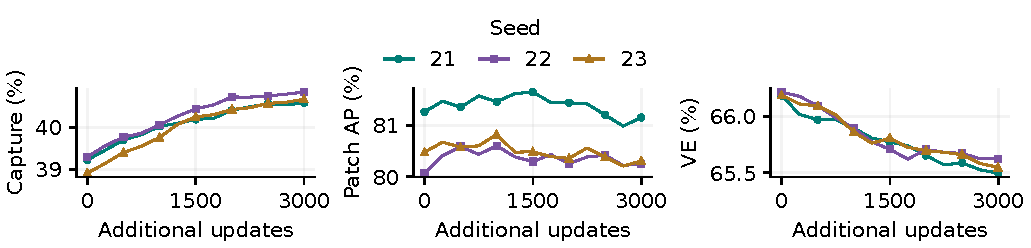
\includegraphics[width=.84\textwidth]{figures/agf_continuation5_curves.pdf}
\caption{Ordinary five-direction continuation: recorded development
checkpoints by seed. These curves are not test scores. Capture increases
while VE declines. AP follows a different trajectory.}
\label{fig:continuation5-curves}
\end{figure*}

Run \texttt{371d2d1d81ea} completes ordinary guided continuation, continued
Vanilla, and a separate gradient-projection trial for the declared training starts.
The five-direction reference is the ordinary GGF arm. It starts from each
completed five-direction checkpoint in Appendix~\ref{app:width5}, retaining
1,024 groups, five directions per group, Top-16 activity (80 coefficient
slots), and 7,869,440 core parameters. Guided models have 150 additional
classifier parameters. Vanilla uses reconstruction alone.

\paragraph{State and matched schedules.}
Each arm adds 3,000 updates at learning rate $3\times10^{-4}$, with noise
scale 0.1 and gradient-norm clipping at five. The model's Adam state,
classifier heads, bounded weight-controller state, loss references, fixed
training-selected readouts, and random-stream state carry forward. Ordinary
guided training continues the weighted objective in Equation~\ref{eq:total}.
Contrast and detection weights remain bounded by 0.40. They are not fixed
at that cap. Reconstruction retains weight one. New image and noise schedules
match by seed, with eight sampled images per update. No warm-up, feature
extraction, readout selection or control retraining occur.
The total scheduled budget is 7,640 reconstruction warm-up updates plus
2,500 and 500 guided updates plus 3,000 continuation updates: 13,640.
The warm-up checkpoint is selected by minimum development MSE, so scheduled
budget does not imply that its chosen weights use the final warm-up step.

\paragraph{Frozen evaluation.}
All nine new endpoints freeze before test scoring. Saved starting reports
and four-direction continued controls are reused without fitting. The same
inspected, coverage-enriched 1,500-image cohort supplies test
scores. No test gradients or new calibration are used.
The archive has 30 model reports (ten arms across training starts), 27 paired
comparisons, and completion records for every new endpoint.

\begin{table*}[t]\centering\small
\caption{Values with $\pm$ show mean and sample SD. Five-direction continuation and equally continued four-direction
controls: means (\%). Passes concern development MSE.}
\label{tab:continuation5-means}
\begin{tabular}{@{}lrrrr@{}}\hline
Model & Capture & AP & VE & Passes\\\hline
GGF 5: start & $39.43\pm0.15$ & $75.04\pm0.42$ & $66.67\pm0.05$ & 3/3\\
GGF 5: continued & $41.04\pm0.11$ & $75.01\pm0.26$ & $66.04\pm0.07$ & 3/3\\
Vanilla 5: continued & $22.34\pm0.52$ & $59.58\pm1.40$ & $68.12\pm0.16$ & 3/3\\
GGF 4: continued & $40.28\pm0.15$ & $75.02\pm0.21$ & $64.83\pm0.01$ & 0/3\\
Vanilla 4: continued & $21.35\pm0.59$ & $57.41\pm0.98$ & $66.74\pm0.05$ & 3/3\\\hline
\end{tabular}\end{table*}

\begin{agfresulttable}
\caption{Five-direction ordinary continuation and its matched Vanilla control:
test percentages by seed. All six pass the original development-MSE limit.}
\label{tab:continuation5-seeds}
\begin{tabular}{@{}rlrrr@{}}\hline
Seed & Model & Capture & AP & VE\\\hline
21 & GGF 5 &40.915&75.303&65.963\\
21 & Vanilla 5 &22.516&58.732&68.026\\
22 & GGF 5 &41.104&74.800&66.103\\
22 & Vanilla 5 &21.751&58.812&68.304\\
23 & GGF 5 &41.093&74.941&66.064\\
23 & Vanilla 5 &22.750&61.191&68.024\\\hline
\end{tabular}\end{agfresulttable}

\paragraph{What improves.}
Against continued width-five Vanilla, GGF gains 18.70 Capture and 15.44
AP points, with positive paired intervals in every run. VE is 2.07 points
lower. Against its own starting checkpoint, it adds 1.60 Capture points,
while AP and VE fall by 0.03 and 0.63 points. Capture intervals are positive
in all seeds. Every AP interval includes zero. Against equally continued
width four, it adds 0.76 Capture and 1.21 VE points, with a mean AP difference
of $-0.002$ points. All Capture intervals are positive, while AP intervals
include zero. This supports Capture gains and similar measured AP, not a
formal equivalence claim. The original development-MSE limit passes in all
five-direction seeds, unlike width-four guided continuation.

\begin{agfresulttable}
\caption{Ordinary five-direction GGF gain intervals on test: conditional
95\% paired image intervals, in percentage points. Each uses 200 draws.}
\label{tab:continuation5-intervals}
\begin{tabular}{@{}rlrr@{}}\hline
Seed & Comparison & Capture interval & AP interval\\\hline
21 & Continued Vanilla 5 &[17.99,18.86]&[15.17,17.76]\\
22 & Continued Vanilla 5 &[18.88,19.86]&[14.60,17.24]\\
23 & Continued Vanilla 5 &[17.91,18.76]&[12.39,14.75]\\\hline
21 & Starting GGF 5 &[1.33,1.54]&[$-0.59$,0.13]\\
22 & Starting GGF 5 &[1.45,1.64]&[$-0.17$,0.45]\\
23 & Starting GGF 5 &[1.72,1.94]&[$-0.33$,0.30]\\\hline
21 & Continued GGF 4 &[0.69,0.88]&[$-0.10$,0.89]\\
22 & Continued GGF 4 &[0.59,0.75]&[$-0.45$,0.27]\\
23 & Continued GGF 4 &[0.74,0.93]&[$-0.86$,0.17]\\\hline
\end{tabular}\end{agfresulttable}



\paragraph{Unadopted optimization trial.}
Weighted PCGrad~\citep{yu2020pcgrad} also projects conflicting task gradients
on encoder and decoder, with an independently saved projection-order stream.
Detection has no decoder gradient. Heads retain their detection gradient,
and the adaptive controller is unchanged. This arm reaches 41.14\% Capture,
74.93\% AP, and 65.95\% VE: 0.11 more Capture than ordinary continuation,
but 0.08 less AP and 0.09 less VE. It does not improve reconstruction and
is not part of our proposed configuration. Full outcomes and implementation
provenance, including this negative result, remain in
\path{evidence/continuation5/}.

These comparisons follow the uncertainty and benchmark-reuse conventions
in Appendix~\ref{app:secondary}.

